%%%%%%%%%%%%%%%%%%%%%%%%%%%
\chapter {General Chordal Rings}
\label{GL}
%%%%%%%%%%%%%%%%%%%%%%%%%%%
Now that we have investigated the problem of disinfecting a network from a  \bv   in   special  classes of chordal rings, we will discuss the problem in general chordal rings, regardless of chord structure.  


The solution  we propose is based on the  idea described for the general chordal ring in Chapter \ref{}, and has already been explained throughout this thesis. In involves an exploration phase, followed by a surrounding phase. Our protocol is based on a general surrounding method that can be applied to any chordal ring structure, regardless of the number or distance of chords. It must be noted that the move-cost for this method is not optimal.

 


 \section{Exploration and Shadowing}
%The main goal of this phase is to determine the location of the original \bv since the location of the \bv is unknown a priori. This process is done by the  exploring team: $LEA$,$EA$, and shadow agent(s) $SA$. 
%Finding the node in which the \bv resides implies creating more \bvs in some cases, destroying $EA$, and clearing that node. As we mentioned before, the technique used in this phase is the {\em safe exploration}.
%\begin{comment}
%Starting from a random node, \hb, $v_0$, the leader and the exploration agent explore the chordal ring
%node by node along the outer ring  (i.e., using only $d_1=1$) in the clockwise direction.  $EA$ moves to the next node $v_{1}$ while $LEA$ waits at $v_{0}$; if $EA$ returns back to its leader, then $v_{1}$ is not a \bv and they both move to $v_{1}$ and so on. However, if $LEA$ receives a \bv instead of $EA$, then the location of the original \bv is detected. 
%\end{comment}
%In order maintain monotonicity, $SH$s are deployed. The deployment of $SH$s starts when $LEA$ and $EA$ have explored at least $d_2$ nodes. 
%\begin{comment}
%In other words, if  $C_n( d_1=1, d_{2}, ..., d_{m})$, and the exploring team currently exploring node $v_j$
%and $\left\vert{S_{area}}\right\vert \ge d_2$, at least one $SA$ is deployed and the number of $SA$s increases as many as the neighbours of the current explored node in the safe area, the number of $SH$s $=|N_{ex}(v_j)|-1$.
%Once $EA$ arrives to the \bv location, it is destroyed, $LEA$ receives a $BV$ instead of EA, that node is cleared, new \bvs are located at all the unprotected(unexplored) neighbours of the original $BV$.
%
%  Since we have a monotone protocol, the explored nodes  in ($S_{area}$) should be protected from potential recontamination. As we mentioned before, the exploring team ($LEA$,$EA$) are moving in clockwise direction along the outer ring, but when they reach a certain node ($v_{n-d_m}$), the possibility of infecting explored node(s) increases; thus, in addition to $SH$s at counter clockwise neighbours, $SH$s are needed at the clockwise neighbours . As we have mentioned before, the area in which the recontamination possibility increases is called danger area  $D_{area}$ where $v_{n-d_m} \leq D_{area}\leq v_{n-1} $.
%\end{comment}
% 
%
%  \begin{center}
%\fbox{
%\begin{minipage}{6 cm}
%{\sc  Exploring and Shadowing}
%  \begin{tabbing}
%  Age\= nts $EA $ and $$LEA$$ at safe node  $v_i$.\\
%\\
% - Compute  $N_{ex}(v_{i+1})$ \\
% - For each $q \in N_{ex}(v_{i+1})$ \\
% \tab  $SH$\ is deployed \\
% - $EA$ moves to $v_{i+1}$\\ \\
% If $EA$ returns back to $v_{i}$\\
% \tab $LEA$ and $EA$ move to $v_{i+1}$\\
% Else (i.e., $BV$ moves to $v_{i}$)\\
%\tab $EA$ is destroyed\\
% \tab $|BV|=N_{un}(v_i)$
%  \end{tabbing}
%\end{minipage}
%}
%\end{center}
%

 The   phase is  described in detail in Chapter \ref{PM}. The following are our observations in general chordal ring structures:

\begin{theorem}

In any  chordal ring $C_n=\{1,d_2,d_3,...,d_m\}$, in the worst case scenario, the \bv is detected in $((2+m)n-2m-3)$ moves.

\end{theorem}
\begin{proof}
The worst case scenario regarding the number of moves required occurs when the \bv  is located at node ($v_{n-1}$) after exploring   $n-1$ nodes.  
 The complexity of this case would be $3n-5$ for the movement of $LEA$ and $EA$, $(\sum\limits_{i=2}^m n-1-d_i)$ for the movement of $SH$s to counter-clockwise neighbours and $(\sum\limits_{i=2}^m d_i-1)$ for $SH$s to clockwise neighbours. 

 In this case, the \bv triggers no new \bvs since all of the neighbouring nodes are occupied by $SH$s, ($2m-1$) $SH$s. This case is considered the worst case scenario in terms of calculating the number of moves, but the best case in terms of cleaning and surrounding agents.
\end{proof}

 
\begin{theorem}

In any  chordal ring $C_n=\{1,d_2,d_3,...,d_m\}$, the worst case scenario regarding the number of agents required for decontamination would occur when $2m-1$ new \bvs are created after triggering the original virus.
\end{theorem}
\begin{proof}
If the \bv is found at node $(v_i)$ where $1\leq v_i< d_2$, the spread of \bvs would be maximixed since no $SH$s have been deployed and the explored neighbours $|N_{ex}(v_i)|=1$, which is $v_{i-1}$ and  is occupied by the  $LEA$. Therefore , the number of unexplored neighbours, o \bvs, is $2m-1$. This number of \bvs requires a high number of surrounding agents. 
\end{proof}



As usual, this phase comes to an end when the \bv is detected and triggered. At this point, new \bvs have been created and moved to the unexplored neighbouring nodes. It is at this point that the second phase begins. 



\section{Surrounding and Eliminating}
 
As described in Chapter \ref{PM}, once the \bv node is detected, the $LEA$ moves to its location and the {\em surrounding and eliminating} phase begins.
%
%  \begin{center}
%\fbox{
%\begin{minipage}{7.5cm}
%{\sc Surrounding and Elimination} 
%  \begin{tabbing}
% $$LEA$$ \= and  $SH$s  covering all $N_{ex}(v)$ \\
% $BV$ comes back from $v$. \\
%  \\
%\>-$SH$s make one move in the clockwise direction.\\
%  \> - Compute  $N_{un}(v)$\\
% \> - For \= each $u \in   N_{un}(v)$:\\
% \>\> Deploy  an  agent  to each  $z\in \{N(u)\setminus  N_{un}(v)\}$\\
% \>\> Wh\=en $N(u)$ is covered:\\
% \>\>\> Deploy one agent to   $u$
%  \end{tabbing}
%\end{minipage}
%}
%\end{center}
%
%

Throughout our study of different classes of chordal rings, we have proposed two routing variations: local and non-local strategies. We have seen in previous chapters that these strategies work for some topologies and not others. For example, the local greedy approach causes incorrect routing in double loop chordal rings and infinite loops in triple-loop and consecutive-chord rings. We can thus deduce that the simple greedy would not work in general chordal rings with arbitrary chord structures (see \ref{no-greedy}). The non-local move-optimal strategy would always work for any chordal rings since this approach requires precise information about the chord structure which is available to the $LEA$ and complex  to calculate. We have observed the following from both strategies:

\begin{itemize}
\item  If node $x_{0}$ represents the location of the original \bv, node $x_{-1}$ is always safe because it is occupied by an agent. This means that it can be used as a starting point to reach any target.
\item After triggering the original {\it black virus}, the new \bvs divide the outer ring into enclosed and open segments. Enclosed segments are areas that include the following set of nodes: $\{ x_{\pm d_i-1}, x_{\pm d_i-2}, x_{\pm d_i-3},..., x_{\pm d_{i\pm1}+1}\}$. Open segments are areas that include the following set of nodes: $\{ x_{\pm d_m\pm1},  x_{\pm d_m\pm2}..., x_{\pm d_m}\}$.
\item Once the agents reach node $x_{\pm d_i-1}$, they are able to reach close targets greedily. In order to avoid getting stuck in infinite loops, agents can reach their close targets by using the one-direction greedy approach. 
\end{itemize} 

%clockwise neighboursEA={ x_{ d_i-1}, x_{d_i-2}, x_{ d_i-3},..., x_{ d_{i-1}+1}}
%counter clockwise neighboursEA={ x_{ -d_i-1}, x_{-d_i-2}, x_{ d_i-3},..., x_{ -d_{i+1}+1}}
Making use of the observations above, we propose an efficient general strategy that is capable of disinfecting any chordal ring and gives upper bounds for the optimal paths.
In this approach, all targets are reached through node $x_{-1}$. The set of targets is calculated based on the location of the original $BV$ and the agents are scattered between $BV$s. The topology is thus divided into {\it enclosed areas} and {\it open areas}.



Note that with respect to node $x_{-1}$, some targets move in a clockwise direction while others move in a counter-clockwise direction.

In order to reach the targets, the $LEA$ deploys agents through $x_{-1}$. The agents then move to the closest neighbour that is greater than or equal to its destination. Once the agent reaches $x_{\pm d_i-1}$, it arrives to the area in which its target resides. The agent then moves greedily in one direction until it reaches its destination. Since this is a one-direction greedy approach, the agent only moves to neighbouring nodes that are greater or equal  to its target. 




  \begin{figure}[h]
\centering
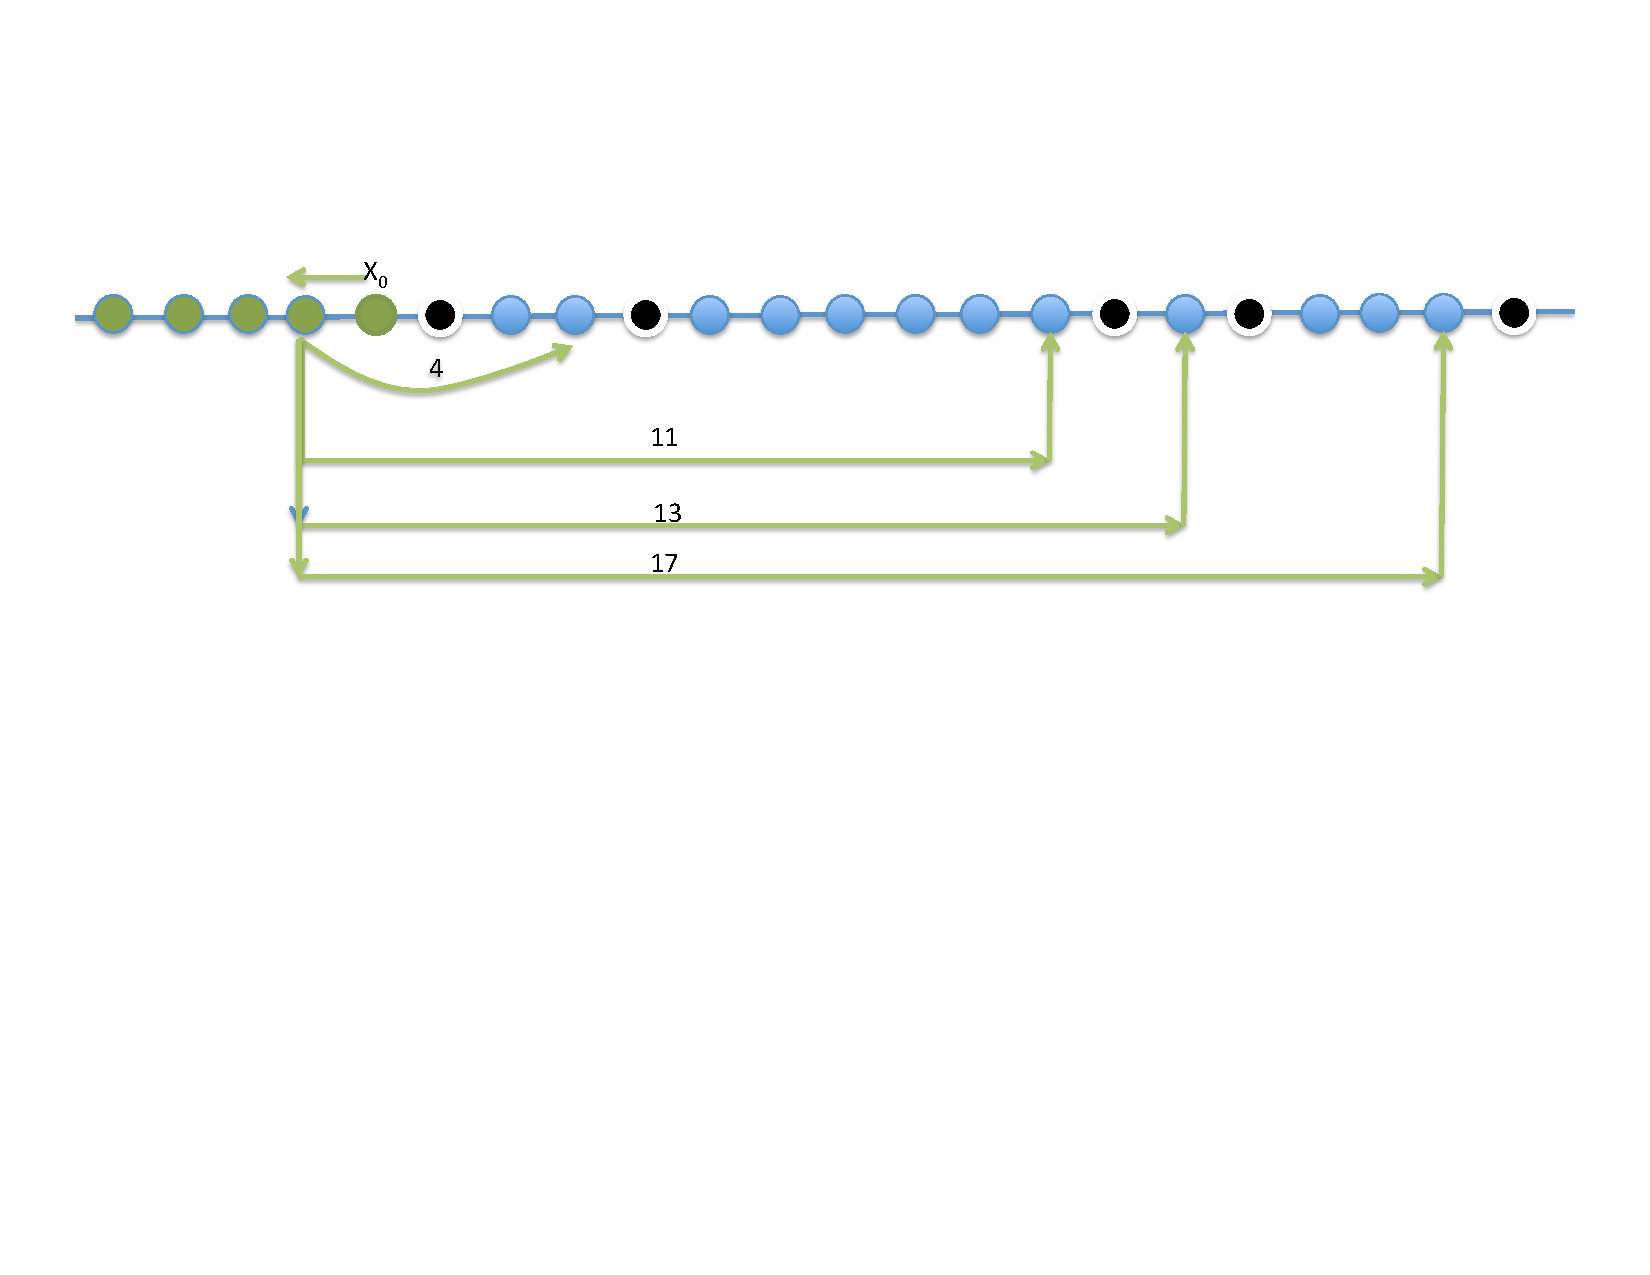
\includegraphics[scale=0.60]{example.pdf}
\caption{Chordal ring C(1,4,11,13,17)}
\label{fig:example}
\end{figure}


 







\begin{center}
\fbox{
\begin{minipage}{7.5 cm}
{\sc General Deployment Strategy}
\begin{tabbing}
Depl\=oying agent $A$ arriving at $x_j$ from $y$ with destination $t$\\ \ \\



If $t =x_{z}$ where $z \in \mathbb{Z}^+ $\\
\tab if  $j=0$\\
 \tab \tab move to $ x_{-1} $ \\ 
\tab if  $j=-1$ \\ 

\tab\tab move to $ x_{d_{i}-1} $ such that  $x_{d_{i}-1} \ge t$ , and $x_{d_{i}-1} $ minimizes $dist(x_{-1},t)$  \\ 

\tab Else\\
\tab\tab if  $t > x_{d_m}$\\
\tab\tab\tab move to $x_{d_m-1}$ then to $x_{2d_{m}-1}$ (i.e., move to the open area)  \\
\tab\tab\tab If $t=x_{2d_{m}}$\\
\tab\tab\tab\tab move to $x_{2d_{m}}$\\
\tab\tab\tab Else\\
\tab\tab\tab compute $next$\\
\tab\tab\tab\tab let $OA=\{ x_{2d_{m}-1},x_{2d_{m}-2},...,x_{d_{m}+1}\}$the open area set \\
\tab\tab\tab\tab  Let $FD =\{ N(x_j)- y- BV \}$ be the set of feasible destinations.\\
\tab\tab\tab\tab let $C=FD  \cap OA$ \\
\tab\tab \tab\tab Agent $A$ moves to $next \in C$ that minimizes $dist(x_j,t)$ and $next \ge t$\\


\tab\tab Else\\

\tab\tab\tab compute $next$\\
\tab\tab\tab\tab let $EA=\{x_{d_i-2},x_{d_i-2}, x_{d_i-3},x_{d_i-4},...,x_{d_{i-1}+1}\}$the enclosed area set \\
\tab\tab\tab\tab  Let $FD =\{ N(x_j)- y - BV \}$ \\%be the set of feasible destinations.\\
\tab\tab\tab\tab let $C=FD  \cap EA$ \\
\tab\tab \tab\tab Agent $A$ moves to $next \in C$ that minimizes $dist(x_j,t)$ and $next \ge t$\\
\\
Else (i.e.,  $t =x_{z}$ where $z \in \mathbb{Z}^- )$\\
\tab if  $j=0$\\
 \tab \tab move to $ x_{-1} $ \\ 
\tab if  $j=-1$ \\ 

\tab\tab move to $ x_{-d_{i}-1} $ such that  $x_{-d_{i}-1} \ge t$ , and $x_{-d_{i}-1} $ minimizes $dist(x_{-1},t)$  \\ % the closest large neighbour of x_{-1} to t

\tab Else\\
\tab\tab if  $t < x_{-d_m}$\\
\tab\tab\tab move to $x_{-d_m-1}$  (i.e., move to the open area)  \\
\tab\tab\tab compute $next$\\
\tab\tab\tab\tab let $OA=\{x_{-d_{m}-1}, x_{-d_{m}-2},x_{-d_{m}-3},...,x_{-2d_{m}}\}$the open area set \\
\tab\tab\tab\tab  Let $FD =\{ N(x_j)- y- BV \}$ \\%be the set of feasible destinations.\\
\tab\tab\tab\tab let $C=FD  \cap OA$ \\
\tab\tab \tab\tab Agent $A$ moves to $next \in C$ that minimizes $dist(x_j,t)$ and $next \ge t$\\


\tab\tab Else\\

\tab\tab\tab compute $next$\\
\tab\tab\tab\tab let $EA=\{x_{-d_i-1},x_{-d_i-2}, x_{-d_i-3},x_{-d_i-4},...,x_{-d_{i+1}+1}\}$the enclosed area set\\
\tab\tab\tab\tab  Let $FD =\{ N(x_j)- y - BV \}$ \\%be the set of feasible destinations.\\
\tab\tab\tab\tab let $C=FD  \cap EA$ \\
\tab\tab \tab\tab Agent $A$ moves to $next \in C$ that minimizes $dist(x_j,t)$ and $next \ge t$\\

   

\end{tabbing}
\end{minipage}
}
\end{center}


\noindent  The following observations were made after using the general strategy:

\begin{theorem}
In any chordal ring $C_(1,d_2,d_3,....d_m)$ with $d_m<<n$, the worst case scenario in terms of number of agents required occurs when triggering the original \bv creates $2m-1$ more {\it black viruses}. In this case,  $size(C)\leq  \lfloor \frac {4m^2-8m+3}{2} \rfloor +6m-1$ and $Spread(C)=2m$.
\end{theorem}

\begin{proof}


In any chordal ring $C$, the worst case scenario occurs when the original \bv is found before deploying any $SH$. In orther words, 
when $|S_{area}|<d_2$. In this case, the maximum number of \bvs would be created: $ 2m-1$ and $\cal BV$ $=\{x_{1}$, $x_{\pm d_2}$, $x_{\pm d_3}$, ..., $x_{\pm d_m}\}$. If we assume that the chords are well separated ( i.e., $d_i-d_{i-1}\ge1$), we have $2(m-1)$ enclosed areas and $2$ open areas. \underline{add a figure here}

Each $bv\in BV$ has at most $2m-1$ neighbours which represent our targets. Some of these are common neighbours or other \bvs, depending on the structure of  the chords. Because we are interested in calculating the $size(C)$, we must first find the number of targets. Each $bv \in BV$ has common neighbours and non-common neighbours. $N_{nc}(bv)$ and $N_{c}(bv)$ denote the set of non-common neighbours and the set of common neighbours of any $bv \in BV$. Note that for any $i$ and $j$, $x_{d_i}+x_{-d_j}$ (a neighbour of node $x_{d_i}$) is the same as $x_{-d_j}+x_{d_i}$ (a neighbour of node $x_{-d_j}$). We have thus found that $|N_{nc}(bv)|\leq2$ and $|N_{c}(bv)|\leq 2m-3$ for any $bv \in BV$. In other words, each \bv has a maximum of two non-common neighbours.  Therefore, we can calculate the maximum possible number of targets as: $|\cal T|$$\leq \lfloor \frac {4m^2-8m+3}{2} \rfloor +4m-2$. $|\cal T|$ represents the number of $SA$s we need to surround the \bvs in the system.
%|N_{nc}(bv)|=2(2m-1), and |N_{nc}(bv)|=((2m-1)(2m-3))/2 floor

The team of agents  consists of $\leq \lfloor \frac {4m^2-8m+3}{2} \rfloor +4m-2$ $SA$s, one $LEA$ and $(2m)$ $CA$s. Thereforem $size(C)\leq  \lfloor \frac {4m^2-8m+3}{2} \rfloor +6m-1$ and $Spread(C)=2m$.

\end{proof}


\begin{theorem}

In any chordal ring  $C_(1,d_2,d_3,....d_m)$ where $\left\vert{S_{area}}\right\vert < x_{d_2}$,  the number of moves required to surround and eliminare $BV$s  is $O(\frac {m^2} { 2})$.
\end{theorem}

\begin{proof}
Calculating the number of moves is not trivial in the general case. This approach is not optimal but it is efficient and gets the routing done correctly. We have an upper bound for the total number of moves required and it is constant. In the analysis of our strategy we find:
\begin{itemize}

\item $2m-1$ targets are reached in $2$ moves, which are $N(x_{-1})$:
$$ x_{0}\xrightarrow {-1}x_{-1} \xrightarrow {\pm d_i} x_{\pm d_i-1}$$

\item Two targets are reached in $4$ moves each which are  $x_{2d_m}$ and $x_{-2d_m}$.
$$ x_{0}\xrightarrow {-1}x_{-1} \xrightarrow {\pm d_m} x_{\pm d_m-1} \xrightarrow {\pm d_m} x_{\pm 2d_m-1}\xrightarrow {\pm 1} x_{\pm 2d_m}$$

\item The rest of targets are nested in the enclosed and open areas and their locations are solely dependent on the chord structure. 
In order to reach them, the agents first move to  node $x_{-1}$ and then to one of the neighbours that satisfies the strategy's conditions. Once an agent is located at the beginning of an interval in which its destination resides, the one-direction greedy strategy begins. 

 The destination between $x_{\pm d_i}$ and $t$ can be minimized if there is a chord $d_i>1$. In our thesis we will consider the worst case scenario in which an agent moves to its target through $\pm 1$ chords. Therefore, each of the other targets, $\leq \lfloor \frac {4m^2-8m+3}{2} \rfloor +2m-3$, are reached in  $O(\frac {m^2} { 2})$ moves.
%$\leq \lfloor \frac {4m^2-8m+3}{2} \rfloor +4m-2  - (2m-1+2)$ (2m-1+2)is the number of the targets we %know exactly how to reach.
%$\cal T$$={t_1,t_2,...,t_j}$
%he  rest targets, $\leq \lfloor \frac {4m^2-8m+3}{2} \rfloor +2m-3$, is reached at most $dist(x_{\pm d_i-1},t_j)$ where $t_j\in$  $\cal T$. Summerizing, the number of moves would be
\end{itemize}
\end{proof}





%
%
%
%
%\subsection{Correctness and Complexity}
%
%For disinfecting any  chordal ring $C_n(d_1=1,d_2,d_3,\ldots d_m)$ with $d_m<<n$, from {\it black viruses}, we have an efficient general algorithm that consists of two phases: {\em Exploring and Shadowing} and {\em Surrounding and Eliminating}. 
%
%\begin{theorem}
%
%The  general algorithm  successfully disinfect any chordal ring from \bvs in a monotone synchronous way. 
%
%\end{theorem}
%
%\begin{proof}
%The correctness of the first phase follows from the fact that the exploring team explores nodes in the outer ring until the original \bv is found, while the monotonicity is achieved because of shadow agents as we discussed before. For the second phase, any $C(d_1=1,d_2,d_3,\ldots d_m)$, the general deployment protocol correctly deliver $SA$s to their targets. 
%The presence of \bvs in the system divides the topology into {\em enclosed} and {\em open} areas as we mentioned before. 
%According to our protocol, the first move done by any $SA$ is moving to $x_{-1}$.  $x_{-1}$ is always safe and its neighbours considered the first nodes in the areas formed by $BV$s. So, when a $SA$ is at $x_{-1}$, it  moves to first node of the area in which its target resides. Then the One-direction greedy strategy starts until the target is reached. Notice that no infinite loops would be formed since the $SA$s approach their targets using the One-direction greedy strategy, see \ref {one-d-noloop}.
%\end{proof}
%
% 


\section{Conclusion}
In this chapter we addressed the {\it black virus disinfection} problem in any general chordal rings, regardless of the chord structure. In this chapter we have been that the first phase remains the same in all chordal rings and that the second phase can be done non-locally. In this case, the $LEA$ finds the shortest paths to the targets and sends $SA$s through them. In order to calculate the complexity of the optimal we require information about the chord structure that is not available. As a result, we propose an efficient protocol that gives us upper bounds to the optimal length. In this protocol we considered some observations from all of the strategies discussed in previous chapters. This protocol is based on the fact that the presence of  \bvs in the system divides the topology into {\em enclosed} and {\em open} areas and that all of those areas are reached through node $x_{-1}$. Once a $SA$ reaches the area in which its target resides, it moves greedily in one direction until it reaches its destination. 

We have found that the total complexity of our general algorithm  in  term of moves is $O(mn)$ for the first phase, where $m$ is the total number of chords in one direction, and $O(\frac {m^2} { 2})$ for the second phase.

%\end{document}




